% Bản tiếng Việt ĐỂ RÀ SOÁT của bài báo (paper_en/main.tex là bản tiếng Anh chính thức; bản này viết lại bằng tiếng Việt để đọc/duyệt, sau đó mới dịch sang tiếng Anh).
% Mọi con số lấy từ các tệp summary.json trong sponge-sim/results (xem phần "Sẵn có dữ liệu và mã"). Các chỗ đỏ "CHƯA CÓ SỐ" là chỗ chưa có dữ liệu.
% Biên dịch: pdflatex main_vi && bibtex main_vi && pdflatex main_vi && pdflatex main_vi (cần gói vietnamese của babel; tham chiếu dùng ../paper_en/references.bib).
\documentclass[12pt,a4paper]{article}
\usepackage[utf8]{inputenc}
\usepackage[T5]{fontenc}
\usepackage[vietnamese]{babel}
\usepackage[margin=2.5cm]{geometry}
\usepackage[numbers,sort&compress]{natbib}
\usepackage{amsmath,amssymb}
\usepackage{booktabs}
\usepackage{tabularx}
\usepackage{array}
\usepackage{enumitem}
\usepackage{microtype}
\usepackage[colorlinks=true,linkcolor=blue,citecolor=blue,urlcolor=blue]{hyperref}
\usepackage{xcolor}
\usepackage{graphicx}
\graphicspath{{../paper_en/figures/}{./}}
\usepackage{tikz}
\usetikzlibrary{arrows.meta,positioning}
\setlength{\parindent}{1.2em}
\setlength{\parskip}{3pt}

\newcommand{\nodata}[1]{\textcolor{red}{[CHƯA CÓ SỐ: #1]}}
\newcommand{\Ntau}{N_{\tau}}

\title{Số lượng ứng viên trước NMS có dự đoán được độ trễ của bộ phát hiện không? Một nghiên cứu đo lường trên lõi CPU được ghim và một nghiên cứu tình huống về tối ưu hóa patch}
\author{Phạm Tuấn Anh$^{1}$, Mai Quốc Bảo$^{1}$, Đinh Phương Nam$^{1,*}$\\
{\small $^{1}$ Trường Đại học Công nghệ Thành phố Hồ Chí Minh (HUTECH)}\\
{\small $^{*}$ Tác giả liên hệ: dp.nam@hutech.edu.vn}}
\date{}

\begin{document}
\maketitle

\begin{abstract}
Các đầu vào đối kháng nhắm vào độ trễ của bộ phát hiện đối tượng thường lấy số hộp ứng viên đi vào bước loại bỏ không cực đại (NMS), ký hiệu $\Ntau$, làm đại lượng cần cực đại hóa, với giả định rằng ứng viên càng nhiều thì pipeline càng chậm. Chúng tôi kiểm tra xem $\Ntau$ có thật sự là một proxy đáng tin cho độ trễ hay không. Chúng tôi xây dựng một giao thức đo gồm: ghim lõi CPU có kiểm chứng dưới tải, đo thời gian theo từng công đoạn, và hiệu chuẩn A/A để cho ra hiệu ứng nhỏ nhất phát hiện được (MDE) của mọi phép so sánh, rồi áp dụng giao thức trên một CPU laptop đã ghim lõi; một điện thoại Arm cũng được chuẩn bị nhưng không ghim được lõi. Một đối chứng dương, trong đó chúng tôi tiêm từ $10^2$ đến $10^4$ ứng viên tổng hợp vào chính pipeline đó, cho thấy độ trễ NMS phụ thuộc vào $\Ntau$, vào cách cài đặt NMS và vào hình học của các hộp. Sau đó, chúng tôi dùng một bộ tối ưu patch bằng thuật toán di truyền làm nghiên cứu tình huống: patch được tối ưu trên 100 ảnh ở độ phân giải 320 và 640 pixel và ở hai ngưỡng điểm, được đo lại theo giao thức đã ghim lõi, và được dùng để kiểm tra một bộ dự đoán chỉ dựa trên $\Ntau$, hiệu chuẩn từ các lần tiêm tổng hợp, dự đoán độ trễ của các tập ứng viên thật tốt đến đâu. Khi tiêm $10^2$ đến $10^4$ ứng viên, độ trễ NMS tăng từ 4 đến 1360 lần tùy cách cài đặt và hình học. Patch từ bộ tối ưu di truyền không làm tăng $\Ntau$ đo được ở 320 px, còn một baseline dùng gradient làm $\Ntau$ tăng 2,3 lần lại để độ trễ toàn trình không đổi trong phạm vi MDE 0,55\% (tỷ số 1,006; khoảng tin cậy 95\% từ 0,997 đến 1,015). Bộ dự đoán chỉ dựa trên $\Ntau$ sai khoảng 5\% với một cách cài đặt NMS và sai khoảng 4 lần với một cách cài đặt khác. Điện thoại không ghim được lõi dưới tải nên bài không có kết quả trên Arm.
\end{abstract}

\noindent\textbf{Từ khóa:} phát hiện đối tượng; loại bỏ không cực đại; đo độ trễ; patch đối kháng; phương pháp đo lường; Arm

\section{Giới thiệu}
Các bộ phát hiện đối tượng dùng NMS tiêu tốn một phần thời gian của mỗi khung hình vào việc loại bỏ các hộp ứng viên chồng lấn nhau. Vì chi phí của NMS tham lam phụ thuộc vào số ứng viên vượt ngưỡng điểm, một hướng nghiên cứu đã chế tác đầu vào sao cho số này tăng lên, nhằm làm chậm quá trình phát hiện \cite{phantom2023,overload2024}, mở rộng ý tưởng chung hơn về các tấn công năng lượng--độ trễ trên mạng nơ-ron \cite{shumailov2021sponge}. Trong các công trình này, số ứng viên $\Ntau$ đóng đồng thời hai vai trò: nó là đại lượng mà bộ tối ưu cực đại hóa, và nó cũng là lời giải thích cho hiện tượng chậm đi quan sát được. Vai trò thứ hai là một khẳng định thực nghiệm, và khẳng định đó có thể sai. Chi phí của NMS còn phụ thuộc vào cách cài đặt và vào cách các hộp ứng viên chồng lấn nhau; hơn nữa NMS chỉ là một công đoạn của pipeline, vốn còn chứa bước lan truyền thuận của mạng.

Bài báo này xem quan hệ giữa $\Ntau$ và độ trễ như một bài toán đo lường và đặt ra bốn câu hỏi.
\begin{description}[leftmargin=2.5em,labelwidth=2.2em,itemsep=2pt]
\item[Q1] Dưới một giao thức đã hiệu chuẩn, độ trễ NMS phụ thuộc vào $\Ntau$ như thế nào khi các ứng viên được kiểm soát, trong khoảng từ $10^2$ đến $10^4$ ứng viên?
\item[Q2] Ở cùng một $\Ntau$, cách cài đặt NMS và hình học của các hộp làm thay đổi độ trễ đó bao nhiêu?
\item[Q3] Với các tập ứng viên do patch đã tối ưu tạo ra trên ảnh thật, $\Ntau$, độ trễ NMS và độ trễ toàn trình thay đổi bao nhiêu so với ảnh sạch, khi so với sàn nhiễu của giao thức?
\item[Q4] Một bộ dự đoán chỉ dựa trên $\Ntau$, được hiệu chuẩn từ các lần tiêm tổng hợp, dự đoán độ trễ NMS của các tập ứng viên thật đó tốt đến đâu?
\end{description}

\paragraph{Đóng góp.}
Chúng tôi đóng góp: (i) một giao thức đo độ trễ pipeline với việc ghim lõi được kiểm chứng dưới tải, đo thời gian theo từng công đoạn, và hiệu chuẩn A/A để báo cáo MDE của mọi phép so sánh; (ii) một đối chứng dương tiêm các ứng viên tổng hợp tại ranh giới đầu ra đã giải mã của một pipeline thật, và vẽ bản đồ độ trễ như hàm của $\Ntau$, cách cài đặt, hình học và giới hạn top-$k$, trên một CPU laptop đã ghim lõi (điện thoại Arm không ghim được dưới tải); (iii) một nghiên cứu tình huống về bộ tối ưu patch kiểu thuật toán di truyền đã công bố, được mở rộng lên 100 ảnh tối ưu, đầu vào 640 pixel và ngưỡng điểm 0,25, kèm các baseline tìm kiếm ngẫu nhiên, đặt vị trí và gradient; (iv) một phép kiểm tra trực tiếp proxy $\Ntau$: sai số dự đoán của một mô hình chỉ dựa trên $\Ntau$ trên các tập ứng viên thật. Giao thức, các giả thuyết và các endpoint được cố định trong một kho mã công khai trước khi tiến hành các phép đo tương ứng.

\paragraph{Bố cục.}
Mục~2 đặt nghiên cứu trong bối cảnh các công trình liên quan; Mục~3 hình thức hóa $\Ntau$ và các đại lượng được so sánh; Mục~4 mô tả giao thức đo, thiết kế đối chứng dương, bộ tối ưu của nghiên cứu tình huống và hồ sơ đăng ký trước; Mục~5 báo cáo các thí nghiệm; Mục~6 thảo luận những gì kết quả cho thấy và không cho thấy; Mục~7 tập hợp các mối đe dọa đối với tính hợp lệ; Mục~8 kết luận.

\section{Công trình liên quan}
\paragraph{Sponge và các tấn công năng lượng--độ trễ.}
Các sponge example làm tăng năng lượng hoặc độ trễ của một mạng bằng các đầu vào được chế tác \cite{shumailov2021sponge}. Với bài toán phát hiện đối tượng, Phantom Sponges chế tác một nhiễu loạn phổ quát làm tăng số hộp đi vào NMS \cite{phantom2023}; Overload tối ưu đầu vào bằng trọng số chú ý không gian và đánh giá trên phần cứng biên \cite{overload2024}; SlowTrack đưa tấn công độ trễ lên chuỗi nhận thức dựa trên camera của hệ thống lái xe \cite{slowtrack2024}. Các tấn công hiệu quả liên quan nhắm vào mô hình sinh chú thích ảnh \cite{nicgslowdown2022} và vào lỗi phần cứng suy luận \cite{bitflip2025}, còn các phòng thủ huấn luyện bộ phát hiện để chịu được tấn công độ trễ \cite{underload2025}. Các công trình ở mức bộ phát hiện dùng số ứng viên, hoặc một đại lượng thay thế gần với nó, làm mục tiêu tối ưu; họ báo cáo mức tăng độ trễ trên mô hình và thiết bị mà họ chọn. Chúng tôi không đề xuất một tấn công mạnh hơn. Chúng tôi kiểm tra chính quan hệ mà mục tiêu tối ưu dựa vào.

\paragraph{Tính thực tiễn của tấn công độ trễ NMS.}
EVADE xem xét liệu các tấn công độ trễ NMS có quan trọng trong triển khai thực tế hay không, có tính đến phần cứng, định dạng mô hình, lượng tử hóa và yêu cầu độ trễ của tác vụ phía sau \cite{evade2025}. Nghiên cứu của chúng tôi bổ sung theo ba hướng. Thứ nhất, nó tách riêng quan hệ giữa ứng viên và độ trễ bằng cách tiêm các tập ứng viên được kiểm soát, tạo ra một đối chứng dương mà các đầu vào do tấn công sinh ra không thể có, vì đầu vào tấn công thay đổi cùng lúc cả ảnh lẫn tập ứng viên. Thứ hai, nó định lượng sàn nhiễu của mỗi phép so sánh bằng thiết kế A/A và báo cáo hiệu ứng so với MDE thay vì chỉ báo tỷ số trần. Thứ ba, nó kiểm tra bộ dự đoán chỉ dựa trên $\Ntau$ trên các tập ứng viên thật và báo cáo chỗ nào bộ dự đoán đúng, chỗ nào sai. EVADE trả lời câu hỏi một tấn công có thực tiễn hay không; chúng tôi trả lời câu hỏi đại lượng đang được tối ưu dự đoán được cái gì và không dự đoán được cái gì.

\paragraph{Patch đối kháng và tối ưu hóa bền vững.}
Patch đối kháng là các nhiễu loạn cục bộ, không phụ thuộc ảnh \cite{brown2017patch}; kỳ vọng trên các phép biến đổi (EOT) tối ưu patch trên các phép biến đổi ảnh ngẫu nhiên để patch chịu được thay đổi kích thước, xoay và biến thiên quang học \cite{athalye2018eot}; patch đã được dùng chống lại các bộ phát hiện người \cite{thys2019fooling}. Bộ tối ưu của nghiên cứu tình huống dùng EOT phần mềm gồm xoay, nhiễu màu, làm mờ và nhiễu, và chèn patch ở dạng số.

\paragraph{Tối ưu hộp đen dựa trên truy vấn.}
Các tấn công hộp đen hiệu quả truy vấn ước lượng hoặc tìm kiếm trên đầu vào chỉ bằng đầu ra của mô hình \cite{ilyas2018blackbox}. Bộ tối ưu của nghiên cứu tình huống dựa trên điểm số theo nghĩa đó: hàm fitness của nó dùng điểm lớp trước NMS của bộ phát hiện và không dùng gradient. Nó không phải một tấn công từ xa bị giới hạn truy vấn, vì nó đọc các điểm trước NMS mà một dịch vụ triển khai thường không trả về; chúng tôi nêu giả định truy cập này ở chỗ mô tả phương pháp.

\paragraph{Đo độ trễ và nhiễu.}
Độ trễ đồng hồ treo tường trên một hệ điều hành đa dụng chịu ảnh hưởng của điều chỉnh tần số, trạng thái nhiệt, hoạt động nền và bộ lập lịch. Báo cáo về mức chậm do tấn công chỉ diễn giải được khi biết độ biến thiên giữa các lần chạy của hệ thống không bị tấn công, và điều này không phải lúc nào cũng được nêu. Do đó chúng tôi mượn một công cụ chuẩn của thực hành thực nghiệm: phép so sánh A/A, trong đó cả hai nhánh là cùng một điều kiện, cho phương sai của hiệu số ghép cặp và từ đó cho hiệu ứng nhỏ nhất mà thiết kế có thể phát hiện. Mọi tỷ số trong bài đều được đọc so với giá trị này.

\paragraph{Bộ phát hiện không có NMS.}
NMS là đặc điểm của các bộ phát hiện dày đặc dựa trên anchor. Các bộ phát hiện dự đoán tập hợp như DETR loại bỏ nó khỏi kiến trúc \cite{carion2020detr}. Các tấn công độ trễ nhắm vào NMS vì thế không thể áp dụng cho các thiết kế này; câu hỏi nghiên cứu ở đây chỉ liên quan đến một họ cụ thể, được triển khai rộng rãi: các bộ phát hiện một giai đoạn kiểu YOLO theo sau là loại bỏ tham lam \cite{redmon2016yolo,neubeck2006nms}.

\begin{table}[t]
\centering\small
\caption{Định vị so với các công trình liên quan gần nhất. Năm dòng đầu tóm tắt những gì mỗi công trình báo cáo ở mức chi tiết liên quan ở đây; dòng cuối mô tả nghiên cứu này.}
\label{tab:related}
\begin{tabularx}{\textwidth}{@{}p{2.8cm}p{3.6cm}p{3.8cm}X@{}}
\toprule
Công trình & Đối tượng & Đại lượng được tối ưu hoặc nghiên cứu & Vai trò của số ứng viên \\
\midrule
Sponge Examples \cite{shumailov2021sponge} & Mạng nơ-ron (nhiều loại dữ liệu) & Năng lượng và độ trễ suy luận & Không riêng cho NMS \\
Phantom Sponges \cite{phantom2023} & Bộ phát hiện có NMS & Số hộp vượt ngưỡng, qua nhiễu loạn phổ quát & Đại lượng tối ưu và lời giải thích cho mức chậm \\
Overload \cite{overload2024} & Bộ phát hiện, phần cứng biên & Độ trễ bộ phát hiện, với trọng số chú ý không gian & Đại lượng tối ưu và lời giải thích cho mức chậm \\
SlowTrack \cite{slowtrack2024} & Chuỗi nhận thức camera cho lái xe & Độ trễ cấp hệ thống qua chuỗi nhiều khung & Không khảo sát ở đây (công trình cấp chuỗi) \\
EVADE \cite{evade2025} & Tấn công độ trễ NMS, triển khai thực tế & Tính thực tiễn trên phần cứng, định dạng, lượng tử hóa, yêu cầu độ trễ & Mục tiêu tấn công đang được đánh giá \\
\textbf{Nghiên cứu này} & Pipeline YOLOv8n, CPU laptop (đã thử Arm) & Quan hệ giữa $\Ntau$ và độ trễ, hiệu chuẩn bằng đối chứng dương và sàn nhiễu A/A & Giả thuyết được kiểm tra \\
\bottomrule
\end{tabularx}
\end{table}

\section{Phát biểu bài toán}
Giả sử một bộ phát hiện sinh ra $A$ anchor cho ảnh $x$, với điểm không phân biệt lớp $s_i(x)=\max_c p_{i,c}(x)$ cho anchor $i$. Số ứng viên tại ngưỡng $\tau$ là
\begin{equation}
\Ntau(x)=\bigl|\{\, i : s_i(x) > \tau \,\}\bigr| .
\end{equation}
Với bộ phát hiện YOLOv8n dùng ở đây, $A=2100$ ở đầu vào $320\times320$ và $A=8400$ ở đầu vào $640\times640$. Độ trễ toàn trình phân rã thành tiền xử lý, lan truyền thuận, giải mã, lọc điểm và NMS:
\begin{equation}
t_{\mathrm{total}} = t_{\mathrm{pre}} + t_{\mathrm{fwd}} + t_{\mathrm{dec}} + t_{\tau} + t_{\mathrm{NMS}} .
\end{equation}
Chỉ $t_{\tau}$ và $t_{\mathrm{NMS}}$ phụ thuộc trực tiếp vào $\Ntau$. Khẳng định proxy được kiểm tra ở đây là: với một pipeline cố định, $\Ntau$ quyết định $t_{\mathrm{NMS}}$, và qua đó quyết định $t_{\mathrm{total}}$. NMS tham lam lặp đi lặp lại việc chọn hộp có điểm cao nhất và loại các hộp chồng lấn với nó, nên chi phí của nó tăng theo số hộp còn được chọn chứ không chỉ theo $\Ntau$ \cite{neubeck2006nms}; vì vậy hình học hộp là một yếu tố đang được kiểm tra chứ không phải nhiễu.

\paragraph{Hiệu ứng so với sàn nhiễu.}
Với phép so sánh hai điều kiện có log-tỷ số ghép cặp theo ảnh $d_i$ ($i=1,\dots,n$) và độ lệch chuẩn mẫu $\hat\sigma_d$, hiệu ứng nhỏ nhất phát hiện được tại mức ý nghĩa $\alpha=0{,}05$ và lực kiểm định $0{,}8$ là
\begin{equation}
\mathrm{MDE}=\bigl(t_{1-\alpha/2,\,n-1}+t_{0.8,\,n-1}\bigr)\,\hat\sigma_d/\sqrt{n},
\end{equation}
được báo cáo dưới dạng phần trăm thay đổi độ trễ. Thí nghiệm A/A, trong đó hai nhánh là cùng một điều kiện, ước lượng $\hat\sigma_d$ cho từng thiết bị, profile và công đoạn. Chúng tôi chỉ diễn giải một tỷ số đo được khi so với MDE này. Khoảng tin cậy chứa 1 không bao giờ được đọc là tương đương.

\subsection{Mô hình chi phí dự đoán điều gì}
Chúng tôi nêu hành vi kỳ vọng của công đoạn NMS trước khi có dữ liệu, để các phép đo có thể bác bỏ nó. NMS tham lam chọn hộp còn lại có điểm cao nhất, loại mọi hộp còn lại có IoU với nó vượt ngưỡng, rồi lặp lại. Gọi $K$ là số hộp được chọn. Một cài đặt vector hóa đơn giản thực hiện $K$ vòng lặp, mỗi vòng duyệt các hộp còn lại, nên chi phí của nó nằm giữa $O(\Ntau)$ (ít hộp được chọn, như ở cụm dày đặc) và $O(\Ntau^2)$ (mọi hộp đều được chọn, như khi các hộp rời nhau). Do đó chi phí phụ thuộc vào hình học thông qua $K$, chứ không chỉ vào $\Ntau$. Các nhân (kernel) của thư viện dùng cùng thuật toán trong mã biên dịch, với hằng số mỗi vòng nhỏ hơn nhiều, và các biến thể NMS theo lớp theo lô dịch chuyển các hộp của mỗi lớp thay vì lặp qua từng lớp. Hai cơ chế khác chặn chi phí trong thực tế: giới hạn số ứng viên đưa vào NMS (top-$k$), khiến $\Ntau$ nhiều nhất là $k$; và giới hạn thời gian bên trong phần hậu xử lý của Ultralytics. Chúng tôi ghi các kỳ vọng như sau và xem xét chúng ở Mục~\ref{sec:results}.
\begin{description}[leftmargin=2.5em,labelwidth=2.2em,itemsep=2pt]
\item[H1] Với một cách cài đặt cố định, độ trễ NMS tăng theo $\Ntau$ trong khoảng $10^2$ đến $10^4$ ứng viên.
\item[H2] Ở cùng $\Ntau$, các hộp rời nhau tốn nhiều hơn các hộp chồng lấn, và khoảng cách lớn nhất ở cài đặt dùng vòng lặp.
\item[H3] Giới hạn top-$k$ làm giảm độ trễ của mọi cách cài đặt khi $\Ntau$ vượt $k$.
\item[H4] Vì $t_{\mathrm{NMS}}$ chỉ là một số hạng của $t_{\mathrm{total}}$, mức tăng của $t_{\mathrm{NMS}}$ chỉ chuyển thành mức tăng toàn trình khi $t_{\mathrm{NMS}}$ chiếm một phần đáng kể của $t_{\mathrm{total}}$.
\end{description}

\section{Giao thức đo}
\subsection{Pipeline và các công đoạn}
Bộ phát hiện là YOLOv8n \cite{jocher2023ultralytics}, một bộ phát hiện một giai đoạn thuộc họ YOLO \cite{redmon2016yolo}, chạy trên PyTorch \cite{paszke2019pytorch}. Pipeline thay đổi kích thước ảnh RGB trực tiếp về kích thước đầu vào của bộ phát hiện mà không thêm viền, chạy mạng ở float32, giải mã đầu ra của head, áp dụng ngưỡng điểm $\tau$ và giới hạn top-$k$ tùy chọn, rồi chạy NMS với ngưỡng IoU 0,45 và tối đa 300 đầu ra. Mỗi công đoạn được đo riêng bằng đồng hồ đơn điệu độ phân giải nano giây, tắt thu gom rác trong vùng đo, sau các lần chạy khởi động bị loại bỏ. Thời gian toàn trình được đo trong một lần gọi và không bao giờ được ghép từ trung vị các công đoạn. Mọi đầu vào là tensor đã chuẩn bị sẵn trong bộ nhớ, nên việc đọc tệp và thu hình từ camera nằm ngoài vùng đo (Hình~\ref{fig:pipeline}).

\begin{figure}[t]
\centering
\begin{tikzpicture}[node distance=3.2mm, every node/.style={font=\scriptsize}, box/.style={draw, rounded corners=1pt, minimum height=5.5mm, inner sep=2pt, align=center}]
\node[box] (a) {Resize};
\node[box, right=of a] (b) {Forward};
\node[box, right=of b] (c) {Decode};
\node[box, right=of c] (d) {$\tau$, cap};
\node[box, right=of d] (e) {NMS};
\draw[-{Stealth[length=1.6mm]}] (a)--(b);
\draw[-{Stealth[length=1.6mm]}] (b)--(c);
\draw[-{Stealth[length=1.6mm]}] (c)--(d);
\draw[-{Stealth[length=1.6mm]}] (d)--(e);
\node[box, below=5mm of c, dashed] (inj) {ứng viên tổng hợp\\($N_\tau$ được kiểm soát)};
\draw[-{Stealth[length=1.6mm]}, dashed] (inj.east) -| (d.south);
\node[above=1.5mm of b, xshift=3mm] {$t_{\mathrm{fwd}}$};
\node[above=1.5mm of d, xshift=2mm] {$t_{\tau}$};
\node[above=1.5mm of e] {$t_{\mathrm{NMS}}$};
\end{tikzpicture}
\caption{Các công đoạn của pipeline được đo riêng. Đường nét đứt là điểm tiêm của đối chứng dương: tập ứng viên tổng hợp thay thế đầu ra đã giải mã và đi vào bộ lọc điểm, nên công đoạn lọc và NMS được đo với $\Ntau$ được kiểm soát.}
\label{fig:pipeline}
\end{figure}

\subsection{Các cách cài đặt NMS}
Bốn cách cài đặt nhận cùng các ứng viên sau ngưỡng. Một vòng lặp PyTorch thuần (không phân biệt lớp) là cài đặt mà mã tối ưu dùng. Hàm \texttt{nms} của torchvision (không phân biệt lớp) và \texttt{batched\_nms} (theo lớp) là các nhân thư viện. Hậu xử lý gốc của Ultralytics, theo lớp và có giới hạn và hạn thời gian riêng, là mặc định của pipeline của chính bộ phát hiện. Trên mẫu hữu hạn không có điểm bằng nhau, các cài đặt trong cùng một nhóm phân biệt lớp giữ cùng tập hộp; điều này được kiểm thử nhưng không được khẳng định cho mọi trường hợp điểm bằng nhau.

\subsection{Thiết bị, ghim lõi và kiểm chứng}
Laptop là Intel Core i5-1335U (hai lõi hiệu năng có SMT và tám lõi tiết kiệm điện) chạy Windows. Thiết bị thứ hai là điện thoại dùng SoC Snapdragon 6 Gen 3 (tám lõi Arm chia hai cụm theo thông số nhà sản xuất), chạy Ubuntu trong môi trường proot trên Android. Tiến trình được ghim vào một CPU logic cho mỗi lõi vật lý. Việc ghim không bao giờ được giả định là hoạt động: với mỗi profile chúng tôi chạy một tải nhân ma trận với số luồng gấp đôi số CPU được phép và yêu cầu (a) thời gian CPU của tiến trình chia cho thời gian treo tường không vượt số CPU được phép, (b) thông lượng ít nhất nửa lõi với profile một lõi, và (c) với điện thoại, ít nhất 99\% các chỉ số CPU chạy gần nhất được lấy mẫu của mọi luồng nằm trong tập được phép. Trên điện thoại, các cụm lõi được nhận diện bằng phép đo tốc độ từng CPU và số luồng mà framework báo cáo không được tin cậy. Profile không qua kiểm chứng thì không được đo.

\subsection{Hiệu chuẩn A/A và kiểm soát nhiệt}
Mỗi profile đo 100 ảnh giữ ra ngoài, mỗi ảnh 20 lần, với hai nhánh gán nhãn A và B theo thứ tự xen kẽ ABBA/BAAB. Log-tỷ số theo ảnh của các trung vị hai nhánh cho $\hat\sigma_d$ và MDE. Một phép đo tham chiếu cố định được chạy lúc bắt đầu phiên, trước mỗi khối và ở cuối, và một khối bị cờ nếu lệch hơn 3\% so với lúc bắt đầu phiên. Trên điện thoại, phép đo được thực hiện theo từng đợt ngắn có nghỉ, các profile được xen kẽ giữa các đợt để nhiệt tích tụ được chia đều, và số khối bị cờ được báo cáo cùng kết quả.

\subsection{Thống kê}
Đơn vị suy luận là ảnh với các phân tích A/A và đáp ứng liều, và là cặp (ảnh, seed patch) với các phân tích patch. Khoảng tin cậy là khoảng phân vị từ 20\,000 lần lấy mẫu lại bootstrap với seed cố định; với phân tích patch, cả ảnh lẫn seed đều được lấy mẫu lại (bootstrap phân vị hai tầng; so sánh với bootstrap theo cụm của \cite{cameron2008cluster}, vốn là bootstrap-$t$ kiểu wild theo cụm và chỉ được trích dẫn cho ý tưởng gom cụm) \cite{efron1979bootstrap}. Tương quan hạng là tương quan Spearman. Những so sánh tạo thành một họ kiểm định giả thuyết sẽ được hiệu chỉnh theo phương pháp Holm \cite{holm1979}; các phân tích ở đây là ước lượng kèm khoảng tin cậy chứ không phải kiểm định. Các phân tích định nghĩa sau khi thấy dữ liệu được gắn nhãn post hoc.

\subsection{Thiết kế đối chứng dương}
Phép tiêm thay đầu ra giải mã của bộ phát hiện bằng một tập ứng viên tổng hợp đi vào bộ lọc điểm và NMS (Hình~\ref{fig:pipeline}). Một tập ứng viên được xác định bởi số anchor $A$, $\Ntau$ mục tiêu, số lớp $n_c$ (80 hoặc 1) và một hình học. Tập rời nhau đặt các hộp trên lưới, mỗi hộp chiếm 80\% ô lưới của nó, để không hai hộp nào chồng lấn (IoU bằng 0) và NMS giữ lại tất cả; đây là trường hợp xấu nhất cho vòng lặp tham lam. Tập cụm dày đặc đặt các hộp cỡ khoảng 48 px, lệch tối đa 2 px, quanh tám tâm, sao cho các hộp trong một cụm chồng lấn với IoU cao hơn ngưỡng và đa số bị loại sớm. Tập hỗn hợp dùng nửa mỗi loại, theo thứ tự ngẫu nhiên. $\Ntau$ ứng viên hoạt động có điểm rút đều từ ngay trên $\tau=0{,}01$ đến một và có lớp ngẫu nhiên; các anchor còn lại của head có điểm dưới $\tau/2$, để đúng $\Ntau$ ứng viên qua bộ lọc. Mọi lần rút đến từ một bộ sinh có seed và mỗi tập đều được băm. Lưới đo gồm ba phần: head của bộ phát hiện 320 px ($A=2100$; $\Ntau\in\{0,10,30,100,300,600,1000,1500,2100\}$, $n_c\in\{80,1\}$), head của bộ phát hiện 640 px ($A=8400$; $\Ntau\in\{0,100,300,1000,3000,8400\}$) và một head tổng hợp với $A=10\,000$ vượt quá mọi head thật, chỉ dùng để đạt $\Ntau=10^4$ ($\Ntau\in\{100,300,1000,3000,10^4\}$). Cả ba hình học, cả hai thiết lập giới hạn (không và 300) và cả bốn cách cài đặt được kết hợp với các lưới này, cho 123 nhóm đo. Mỗi nhóm được đo 30 lần sau 3 lần khởi động bị loại; thứ tự các cách cài đặt trong một khối theo thiết kế vuông Latin, và 12 nhóm tạo thành một khối bắt đầu bằng một phép đo tham chiếu. Ngưỡng IoU là 0,45. Một phép thử riêng tiêm $\Ntau\in\{0,100,300,1000,2100\}$ hộp rời nhau vào toàn bộ pipeline của một ảnh cố định, cho cài đặt PyTorch thuần và cài đặt Ultralytics, mỗi loại 20 lần lặp, và đếm số lần lặp vượt mốc 100~ms (một giá trị do các tác giả chọn để tham chiếu, không phải yêu cầu của một ứng dụng nào).

\subsection{Đặc tả bộ tối ưu của nghiên cứu tình huống}
Bảng~\ref{tab:spec} liệt kê các thiết lập của bộ tối ưu. Các patch ứng viên được chấm điểm trên một tập huấn luyện cố định gồm 100 ảnh huấn luyện COCO \cite{lin2014coco} với EOT phần mềm (xoay, nhiễu màu, làm mờ và nhiễu; một lần rút cho mỗi lần đánh giá). Ngân sách tính bằng số lượt lan truyền thuận ứng viên--ảnh: 10\,000, 25\,000 và 62\,500, tương ứng 100, 250 và 625 lần đánh giá ứng viên trên 100 ảnh; mốc cuối cùng là mốc được phân tích, hai mốc trước được giữ lại để cho thấy sự bão hòa. Vị trí patch là cửa sổ có phương sai Laplacian lớn nhất của mỗi ảnh (đặt theo độ nổi bật), trừ các baseline đặt vị trí. Các patch được sinh trên GPU (Tesla V100) vì chi phí CPU của toàn bộ ngân sách trên mười seed là quá lớn; do bộ sinh số ngẫu nhiên của GPU và CPU khác nhau, các patch không trùng từng byte với những gì mã CPU sẽ tạo ra, và giá trị băm của mỗi patch đã lưu là căn cứ cho những gì được đo. Baseline gradient dùng tham số hóa tanh của patch và leo dốc trung bình trên các ảnh của $\sum_i \tanh(s_i)$ theo các pixel patch; nó cần gradient xuyên qua bộ phát hiện nên là một tham chiếu hộp trắng.

\begin{table}[t]
\centering\small
\caption{Thiết lập của các điều kiện trong nghiên cứu tình huống. $\tau_{\mathrm{obj}}$ là ngưỡng trong hàm mục tiêu tối ưu. Mọi điều kiện dùng 100 ảnh huấn luyện, EOT phần mềm, mười seed (0--9) và cùng ba mức ngân sách.}
\label{tab:spec}
\begin{tabular}{@{}llccc@{}}
\toprule
Điều kiện & Phương pháp & Đầu vào (px) & Patch (px) & $\tau_{\mathrm{obj}}$ \\
\midrule
C1 & GA, đặt theo độ nổi bật & 320 & 64 & 0,01 \\
C2 & GA, đặt theo độ nổi bật & 640 & 128 & 0,01 \\
C3 & GA, đặt theo độ nổi bật & 320 & 64 & 0,25 \\
C4 & GA, đặt theo độ nổi bật & 640 & 64 & 0,01 \\
B1 & GA, đặt ở tâm & 320 & 64 & 0,01 \\
B2 & GA, đặt ngẫu nhiên & 320 & 64 & 0,01 \\
B3 & tìm kiếm ngẫu nhiên, độ nổi bật & 320 & 64 & 0,01 \\
B4 & leo gradient (tanh) & 320 & 64 & 0,01 \\
\bottomrule
\end{tabular}
\end{table}

\subsection{Đăng ký trước và các sai lệch}
Giả thuyết, endpoint và quy tắc quyết định của mỗi thí nghiệm được viết trong một tệp đăng ký trước và cố định bằng một tag quản lý phiên bản trước khi tiến hành phép đo tương ứng (các tag cho đối chứng dương, giao thức điện thoại, đo lại patch và sinh patch được đặt cùng lúc; phụ lục bổ sung cho đường cơ sở 640 px có tag riêng). Các sai lệch so với kế hoạch được liệt kê trong Bảng~\ref{tab:dev} và trong kho mã; không sai lệch nào thay đổi endpoint hay quy tắc quyết định sau khi đã thấy dữ liệu, ngoại trừ việc thêm một đối chứng còn thiếu, mà bản thân việc đó cũng được báo cáo như một sai lệch.

\begin{table}[t]
\centering\small
\caption{Các sai lệch và kết quả âm của nghiên cứu. Mọi bản ghi thô, kể cả những bản bị loại, đều được giữ trong kho mã.}
\label{tab:dev}
\begin{tabularx}{\textwidth}{@{}lX@{}}
\toprule
Mục & Điều đã xảy ra và cách xử lý \\
\midrule
Các lần A/A đầu & Hai lần thử A/A trước đó không hợp lệ; chúng được giữ nhưng không dùng. Lần A/A được phân tích là lần thứ ba. \\
Thời điểm phân tích A/A & Script phân tích được khởi chạy trên một phép đo vẫn đang chạy; bản tóm tắt một phần bị loại bỏ và phân tích được lặp lại sau khi phép đo kết thúc. \\
Drift của phép đo tham chiếu & Lần A/A có 2/11 điểm tham chiếu bị cờ drift, đối chứng dương 2/12, và lần đo lại patch 0/11; các khối bị cờ vẫn nằm trong phân tích chính. \\
Lỗi backend tại $\Ntau=6$ & Lần đo lại patch đầy đủ đầu tiên dừng khi một tập ứng viên có đúng sáu hộp bị hậu xử lý của Ultralytics hiểu nhầm là đầu ra end-to-end. Cách dựng đầu vào được sửa, một kiểm thử hồi quy được thêm, và toàn bộ lần đo lại được lặp; lần chạy bị dừng được giữ. \\
Thiếu đường cơ sở 640 px & Lần đo lại patch không có nhánh sạch 640 px nên kết quả 640 px không đọc được. Một phụ lục thêm nhánh này, kèm A/A ở 640 px, và được gắn tag trước khi đo. \\
Điện thoại & Không kiểm chứng được việc ghim lõi dưới tải trên cả hai cụm lõi của thiết bị; không có phép đo thời gian nào được thực hiện và không có kết quả điện thoại nào được báo cáo. \\
\bottomrule
\end{tabularx}
\end{table}

\section{Thí nghiệm}
\label{sec:results}
\subsection{Hiệu chuẩn giao thức (A/A)}
Bảng~\ref{tab:aa} báo cáo MDE của từng công đoạn trên profile laptop đã ghim lõi (CPU logic 2, một luồng torch; số lõi hiệu dụng 0,91 dưới tải) ở hai độ phân giải. Ở 320 px, MDE toàn trình là 0,55\%, và MDE của các công đoạn NMS là 0,64\% (PyTorch thuần) và 1,1\% (torchvision). Hai trong 11 điểm tham chiếu của lần chạy này vượt cờ drift 3\% (khối 1 và 3, thay đổi lớn nhất 26\%); loại hai khối bị cờ còn lại 80 ảnh, và chênh lệch A/A toàn trình vẫn nằm trong khoảng $\pm0{,}5\%$ (khoảng tin cậy 95\% của log-tỷ số trung bình từ $-0{,}0038$ đến $0{,}0046$). Ở 640 px, việc ghim lõi cũng qua kiểm chứng (số lõi hiệu dụng 0,76), nhưng sàn nhiễu cao hơn rõ rệt: MDE toàn trình là 1,9\% và 8 trong 11 điểm tham chiếu bị cờ drift (thay đổi lớn nhất 18\%), nên khi loại các khối bị cờ chỉ còn 30 ảnh và khoảng tin cậy của log-tỷ số toàn trình rộng ($-0{,}035$ đến $0{,}023$). Nguyên nhân của drift cao ở lần chạy này chưa được xác định; trong khi đo có các tác vụ soạn thảo nhẹ chạy song song trên cùng máy, và chúng tôi không thể loại trừ ảnh hưởng của chúng. Vì vậy MDE 640 px phải đọc như một cận trên thận trọng của độ nhạy, không phải một sàn nhiễu sạch. Các profile A/A khác dự kiến (lõi tiết kiệm điện của laptop, điện thoại) không có: điện thoại không qua kiểm chứng ghim lõi (Mục~\ref{sec:phone}).

\begin{table}[t]
\centering\small
\caption{Hiệu chuẩn A/A trên profile laptop đã ghim lõi: hiệu ứng nhỏ nhất phát hiện được (MDE, \%) và thời gian trung vị mỗi công đoạn, 100 ảnh $\times$ 20 lần lặp, ở hai độ phân giải đầu vào. Các điểm tham chiếu bị cờ drift vẫn nằm trong phân tích.}
\label{tab:aa}
\begin{tabular}{@{}lcccc@{}}
\toprule
 & \multicolumn{2}{c}{320 px} & \multicolumn{2}{c}{640 px} \\
\cmidrule(lr){2-3}\cmidrule(lr){4-5}
Công đoạn & MDE (\%) & Trung vị (ms) & MDE (\%) & Trung vị (ms) \\
\midrule
Tiền xử lý & 1,0 & 5,60 & 1,6 & 10,5 \\
Lan truyền thuận & 0,69 & 45,8 & 1,7 & 180 \\
Lọc điểm ($\tau$) & 1,0 & 0,066 & 1,5 & 0,108 \\
NMS (PyTorch thuần) & 0,64 & 1,14 & 2,4 & 1,48 \\
NMS (torchvision) & 1,1 & 0,101 & 1,3 & 0,120 \\
Toàn trình & 0,55 & 53,5 & 1,9 & 199 \\
Điểm tham chiếu bị cờ / tổng & 2/11 & & 8/11 & \\
\bottomrule
\end{tabular}
\end{table}

\subsection{Đối chứng dương: tiêm ứng viên tổng hợp}
Trên profile laptop đã ghim lõi, NMS PyTorch thuần với 2100 ứng viên rời nhau mất 252~ms so với 0,89~ms với 10 ứng viên, tức tỷ số 281 (khoảng tin cậy 95\% từ 278 đến 285), vượt xa $1+\mathrm{MDE}$. Mọi lần lặp toàn trình của pipeline PyTorch thuần với 2100 ứng viên được tiêm (20 trên 20; khoảng Wilson 95\% từ 0,84 đến 1,0) đều vượt mốc tham chiếu 100~ms, vốn là giá trị do các tác giả chọn. Sự phụ thuộc vào $\Ntau$ giữa $10^2$ và $10^4$ được phát hiện ở cả bốn cách cài đặt và cả ba hình học ở độ nhạy này (cận dưới của các khoảng tin cậy xa hơn nhiều so với $1+\mathrm{MDE}$), nhưng độ lớn của nó thay đổi hai bậc độ lớn theo cách cài đặt và hình học (Bảng~\ref{tab:dose}). Với cụm dày đặc, PyTorch thuần chỉ tăng 4,0 lần, phù hợp với việc đa số hộp bị loại sớm, trong khi \texttt{nms} của torchvision tăng 22,5 lần; với các hộp rời nhau, các tỷ số là 225 và 1360.

\begin{table}[t]
\centering\small
\caption{Tỷ số độ trễ NMS tại $\Ntau=10^4$ so với $\Ntau=10^2$ (không phân biệt lớp, 80 lớp, không giới hạn), chỉ trên laptop; điện thoại không được đo.}
\label{tab:dose}
\begin{tabular}{@{}llcc@{}}
\toprule
Cách cài đặt & Hình học & Tỷ số (laptop) & Khoảng tin cậy 95\% \\
\midrule
PyTorch thuần & rời nhau & 225 & 221 đến 231 \\
PyTorch thuần & cụm dày đặc & 4,0 & 3,9 đến 4,2 \\
\texttt{nms} của torchvision & rời nhau & 1360 & 1250 đến 1410 \\
\texttt{nms} của torchvision & cụm dày đặc & 22,5 & 20,8 đến 23,5 \\
\bottomrule
\end{tabular}
\end{table}

\begin{figure*}[t]
\centering
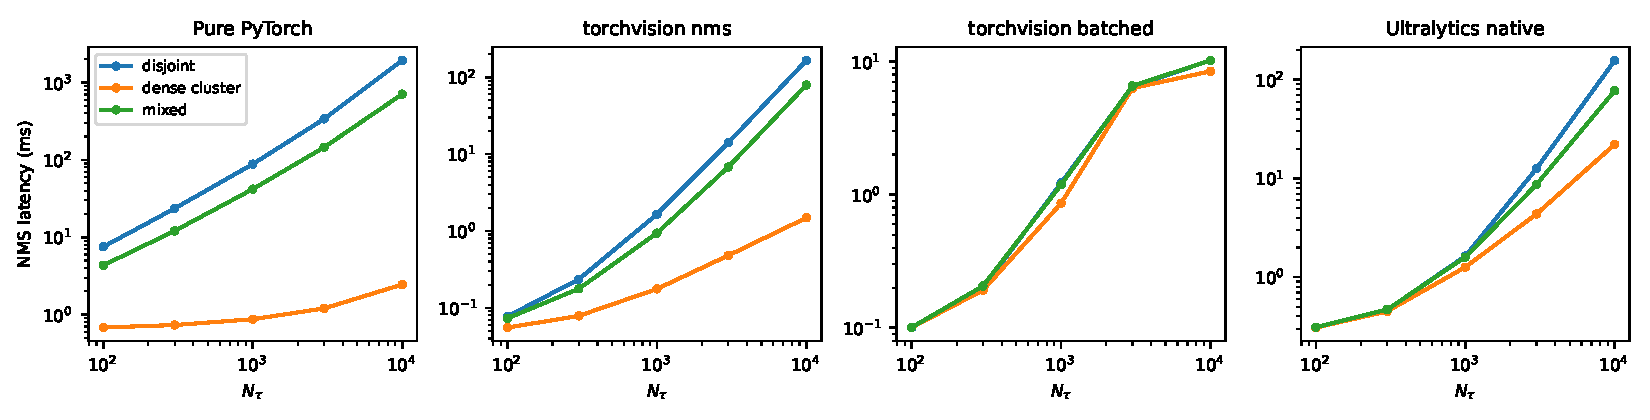
\includegraphics[width=\textwidth]{fig2_dose_response.pdf}
\caption{Độ trễ NMS theo $\Ntau$ trên profile laptop đã ghim lõi (lưới 10\,000 anchor, 80 lớp, không giới hạn) cho bốn cách cài đặt và ba hình học hộp. Đường là trung vị; dải tô màu là khoảng tin cậy bootstrap 95\% theo các lần lặp. Cả hai trục đều là thang logarit.}
\label{fig:dose}
\end{figure*}

\subsection{Cách cài đặt, hình học, số lớp và giới hạn top-$k$}
\paragraph{Cách cài đặt và hình học ở cùng $\Ntau$ (H2).}
Tại $\Ntau=300$ trên head 2100 anchor với hình học hỗn hợp, NMS PyTorch thuần chậm hơn \texttt{nms} của torchvision 80 lần (tỷ số 80,3; khoảng tin cậy từ 76,4 đến 81,9), NMS gốc Ultralytics chậm hơn 2,9 lần (2,92; từ 2,79 đến 2,98), và \texttt{batched\_nms} của torchvision chậm hơn 1,3 lần (1,33; từ 1,24 đến 1,36). Hình học quan trọng không kém cách cài đặt. Tại $\Ntau=2100$, các hộp rời nhau tốn gấp 192 lần cụm dày đặc ở vòng lặp PyTorch thuần (khoảng tin cậy từ 189 đến 196), gấp 13 lần ở \texttt{nms} của torchvision (12,9 đến 14,7), gấp 1,8 lần ở cài đặt Ultralytics (1,74 đến 1,82), và không nhiều hơn ở \texttt{batched\_nms} của torchvision (1,01; từ 0,89 đến 1,07). Vì vậy ở cùng $\Ntau$, chi phí NMS có thể khác nhau hơn hai bậc độ lớn; đó là lý do cách cài đặt và hình học được báo cáo riêng xuyên suốt bài.

\paragraph{Tốc độ tăng mô tả.}
Bảng~\ref{tab:slopes} cho độ dốc của đường cong log--log trên $\Ntau\ge100$ với head 10\,000 anchor. Độ dốc gần một phù hợp với mức tăng tỷ lệ với $\Ntau$ và độ dốc lớn hơn một phù hợp với mức tăng nhanh hơn, nhưng chúng tôi không suy ra lớp độ phức tạp từ sáu mức; bảng chỉ mô tả đường cong đã đo. Đường cong cụm dày đặc của vòng lặp PyTorch thuần gần như phẳng (độ dốc 0,30), trong khi \texttt{nms} của torchvision trên các hộp rời nhau tăng với độ dốc 1,59.

\begin{table}[t]
\centering\small
\caption{Độ dốc log--log của độ trễ NMS theo $\Ntau$ trên các mức đã đo $\ge 100$ (head 10\,000 anchor, 80 lớp, không giới hạn); khoảng tin cậy bootstrap 95\% trong ngoặc. Chỉ mang tính mô tả.}
\label{tab:slopes}
\begin{tabular}{@{}lccc@{}}
\toprule
Cách cài đặt & Rời nhau & Cụm dày đặc & Hỗn hợp \\
\midrule
PyTorch thuần & 1,17 [1,17; 1,17] & 0,30 [0,29; 0,32] & 1,07 [1,05; 1,08] \\
\texttt{nms} của torchvision & 1,59 [1,58; 1,60] & 0,69 [0,67; 0,69] & 1,42 [1,40; 1,45] \\
torchvision theo lô & 1,09 [1,08; 1,10] & 1,08 [1,07; 1,09] & 1,07 [1,05; 1,08] \\
Ultralytics gốc & 1,29 [1,29; 1,30] & 0,96 [0,95; 0,97] & 1,21 [1,20; 1,21] \\
\bottomrule
\end{tabular}
\end{table}

\paragraph{Số lớp.}
Các cài đặt không phân biệt lớp không bị ảnh hưởng bởi số lớp, đúng như kỳ vọng: tại $\Ntau=2100$ với hình học hỗn hợp, thời gian trung vị của NMS PyTorch thuần là 114,6~ms với 80 lớp và 116,5~ms với một lớp, còn của \texttt{nms} torchvision là 1,85 và 1,85~ms. Các cài đặt phân biệt lớp nhanh hơn khi chỉ có một lớp, vì các hộp thuộc lớp khác nhau không còn phải tách bằng phép dịch hoặc vòng lặp theo lớp: \texttt{batched\_nms} của torchvision mất 6,35~ms với 80 lớp và 2,16~ms với một lớp, và cài đặt Ultralytics lần lượt 4,45 và 2,39~ms. Do đó một bộ phát hiện phân biệt lớp có nhiều lớp thể hiện sự phụ thuộc vào $\Ntau$ khác với bộ phát hiện một lớp, và một phép so sánh chuẩn chỉ với một lớp sẽ đánh giá thấp sự phụ thuộc đó.

\paragraph{Giới hạn top-$k$ (H3).}
Bảng~\ref{tab:cap} cho độ trễ NMS trung vị tại $\Ntau=10^4$ khi không có giới hạn và khi giới hạn 300 ứng viên. Giới hạn loại bỏ phần lớn chi phí: với các hộp rời nhau, vòng lặp PyTorch thuần giảm từ 2129 xuống 29,6~ms, \texttt{nms} của torchvision từ 137 xuống 0,21~ms, và cài đặt Ultralytics từ 140 xuống 0,54~ms. Việc chọn 300 điểm cao nhất thuộc công đoạn lọc điểm, vốn mất khoảng 0,29~ms tại $\Ntau=10^4$ khi không có giới hạn và 0,39~ms khi có giới hạn đối với nhánh PyTorch thuần. Một pipeline triển khai có giới hạn số ứng viên trước NMS sẽ chặn lợi ích mà việc tăng $\Ntau$ có thể mang lại, bất kể bộ tối ưu là gì.

\begin{table}[t]
\centering\small
\caption{Độ trễ NMS trung vị (ms) tại $\Ntau=10^4$ (head 10\,000 anchor, 80 lớp) khi không có giới hạn và khi giới hạn 300 ứng viên.}
\label{tab:cap}
\begin{tabular}{@{}llcc@{}}
\toprule
Hình học & Cách cài đặt & Không giới hạn & Giới hạn 300 \\
\midrule
Rời nhau & PyTorch thuần & 2129 & 29,6 \\
 & \texttt{nms} của torchvision & 137 & 0,210 \\
 & torchvision theo lô & 12,0 & 0,244 \\
 & Ultralytics gốc & 140 & 0,542 \\
Hỗn hợp & PyTorch thuần & 775 & 15,2 \\
 & \texttt{nms} của torchvision & 95,4 & 0,184 \\
 & torchvision theo lô & 12,5 & 0,255 \\
 & Ultralytics gốc & 110 & 0,564 \\
Cụm dày đặc & PyTorch thuần & 3,31 & 0,904 \\
 & \texttt{nms} của torchvision & 1,54 & 0,102 \\
 & torchvision theo lô & 9,88 & 0,229 \\
 & Ultralytics gốc & 26,7 & 0,527 \\
\bottomrule
\end{tabular}
\end{table}

\subsection{Tiêm vào toàn bộ pipeline (H4)}
Bảng~\ref{tab:pipe} báo cáo độ trễ toàn trình của pipeline đầy đủ cho một ảnh cố định khi tiêm các tập ứng viên rời nhau. Với NMS PyTorch thuần, thời gian trung vị tăng từ 44,9~ms khi không tiêm ứng viên lên 303~ms ở 2100, và từ 1000 ứng viên trở đi cả 20 lần lặp đều vượt mốc tham chiếu 100~ms. Với cài đặt Ultralytics, trung vị chỉ tăng từ 45,6 lên 55,0~ms và không lần lặp nào vượt mốc. Bước lan truyền thuận mất khoảng 45~ms, nên phép tiêm chỉ đẩy thời gian toàn trình lên đáng kể khi cài đặt NMS đủ chậm để cạnh tranh với bước lan truyền thuận. Lần lặp duy nhất vượt mốc ở mức 100 ứng viên, ở cả hai cách cài đặt, là một điểm ngoại lai về thời gian chứ không phải hiệu ứng liều: trung vị ở mức đó là 54,0 và 45,8~ms.

\begin{table}[t]
\centering\small
\caption{Độ trễ toàn trình của pipeline đầy đủ theo số ứng viên rời nhau được tiêm (một ảnh, 20 lần lặp). Trung vị tính bằng ms; số lần lặp vượt mốc tham chiếu 100~ms trong ngoặc.}
\label{tab:pipe}
\begin{tabular}{@{}rcc@{}}
\toprule
$\Ntau$ được tiêm & PyTorch thuần & Ultralytics gốc \\
\midrule
0 & 44,9 (0) & 45,6 (0) \\
100 & 54,0 (1) & 45,8 (1) \\
300 & 75,3 (0) & 46,9 (0) \\
1000 & 154 (20) & 49,7 (0) \\
2100 & 303 (20) & 55,0 (0) \\
\bottomrule
\end{tabular}
\end{table}

\subsection{Nghiên cứu tình huống: bộ tối ưu patch bằng thuật toán di truyền}
\paragraph{Bộ tối ưu.}
Bộ tối ưu của nghiên cứu tình huống đặt một patch ghi đè $64\times64$ tại cửa sổ có phương sai Laplacian lớn nhất của mỗi ảnh và tiến hóa các pixel của nó bằng thuật toán di truyền (quần thể 20, năm cá thể ưu tú, lai ghép tách ngang, đột biến Gauss) dưới EOT phần mềm. Hàm fitness là $\sum_i s_i \mathbb{1}[s_i>\tau]+\lambda \Ntau$ với $\lambda=1{,}5$, chỉ tính từ các điểm lớp trước NMS. Nó không chứa thành phần độ trễ nào và không dùng gradient. Đây chính là đại lượng mà quan hệ với độ trễ đang được nghiên cứu.

\paragraph{Quy mô.}
Các lần chạy trước đây tối ưu trên bốn ảnh. Ở đây tập tối ưu có 100 ảnh (một mẫu cố định, có seed, từ một tập con của tập huấn luyện COCO \cite{lin2014coco}), tách rời khỏi 100 ảnh giữ ra ngoài dùng để đo. Các điều kiện gồm: $320$ px với patch $64$ px ($4\%$ diện tích) tại $\tau=0{,}01$; $640$ px với patch $128$ px (cùng tỷ lệ diện tích); $320$ px với ngưỡng mục tiêu $\tau=0{,}25$; và, như một điều kiện phụ, $640$ px với patch $64$ px ($1\%$ diện tích). Mỗi điều kiện dùng mười seed tối ưu và cùng số lần đánh giá ứng viên như các lần chạy trước.

\paragraph{Các baseline.}
Chúng tôi đưa vào tìm kiếm ngẫu nhiên với đặt vị trí theo độ nổi bật, thuật toán di truyền với đặt vị trí ở tâm, thuật toán di truyền với đặt vị trí ngẫu nhiên, và một baseline leo gradient theo điểm số được điều chỉnh từ Overload \cite{overload2024}. Baseline gradient là một sự điều chỉnh cho patch ghi đè cục bộ và không phải một bản tái hiện của bản gốc.

\paragraph{Phép đo.}
Các patch được đóng băng bằng SHA-256 trước khi đo. Các ảnh giữ ra ngoài, có và không có mỗi patch, được đo trên profile đã ghim lõi: $\Ntau$ tại $\tau\in\{0{,}01;0{,}25\}$, các công đoạn lọc điểm và NMS cho bốn cách cài đặt, và độ trễ toàn trình cho hai cách cài đặt.

\paragraph{Kết quả tối ưu trên tập huấn luyện.}
Bảng~\ref{tab:train} cho fitness huấn luyện tốt nhất đạt được ở mỗi mức ngân sách, lấy trung bình trên mười seed. Giá trị fitness phụ thuộc vào ngưỡng và kích thước đầu vào, nên có thể so sánh trong một nhóm cột cùng đầu vào và ngưỡng chứ không so được giữa các nhóm. Thuật toán di truyền bão hòa sớm: với C1, fitness tốt nhất trung bình tăng từ 185,1 ở 10\,000 lượt lên 186,6 ở 62\,500 lượt, tức tăng 0,8\%. Ở mức ngân sách cuối, tìm kiếm ngẫu nhiên với cùng cách đặt vị trí đạt 186,0, chỉ thấp hơn thuật toán di truyền 0,6, trong khi hai baseline đặt vị trí cao hơn (đặt ở tâm 191,0; đặt ngẫu nhiên 193,5), nên trên tập huấn luyện này lựa chọn vị trí đặt làm fitness thay đổi nhiều hơn quy trình tìm kiếm. Baseline gradient cao hơn xa mọi điều kiện không dùng gradient (334,1), đúng như kỳ vọng với một phương pháp hộp trắng dùng gradient của chính hàm mục tiêu. Thời gian đồng hồ trên GPU cho một seed và toàn bộ ngân sách là 30~s ở 320 px với các điều kiện không dùng gradient, 97 đến 98~s ở 640 px, và 86~s với baseline gradient.

\begin{table}[t]
\centering\small
\caption{Fitness huấn luyện tốt nhất (trung bình trên mười seed, độ lệch chuẩn trong ngoặc) ở ba mức ngân sách (lượt lan truyền thuận ứng viên--ảnh).}
\label{tab:train}
\begin{tabular}{@{}lccc@{}}
\toprule
Điều kiện & 10\,000 & 25\,000 & 62\,500 \\
\midrule
C1 (320 px, $\tau_{\mathrm{obj}}$ 0,01) & 185,1 (1,7) & 185,9 (1,2) & 186,6 (1,6) \\
C3 (320 px, $\tau_{\mathrm{obj}}$ 0,25) & 39,8 (0,2) & 40,0 (0,3) & 40,5 (0,3) \\
C2 (640 px, patch 128 px) & 294,4 (3,9) & 295,5 (2,9) & 297,3 (2,2) \\
C4 (640 px, patch 64 px) & 299,4 (1,3) & 301,4 (1,9) & 303,1 (1,7) \\
B1 (đặt ở tâm) & 188,7 (1,5) & 189,8 (1,0) & 191,0 (1,4) \\
B2 (đặt ngẫu nhiên) & 191,6 (1,9) & 193,1 (1,5) & 193,5 (1,9) \\
B3 (tìm kiếm ngẫu nhiên) & 184,5 (0,8) & 185,1 (0,8) & 186,0 (1,0) \\
B4 (gradient, tanh) & 218,1 (14,9) & 314,4 (12,8) & 334,1 (11,6) \\
\bottomrule
\end{tabular}
\end{table}

\paragraph{Kết quả đo lại.}
Các patch được sinh trên GPU, đóng băng bằng giá trị băm và đo trên profile laptop đã ghim lõi (số lõi hiệu dụng 0,84 dưới tải; 0 trên 11 điểm tham chiếu bị cờ drift; MDE toàn trình 0,55\%). Bảng~\ref{tab:patches} cho tỷ số của ảnh có patch so với ảnh sạch ở 320 px. Có ba phát hiện đáng chú ý.

Thứ nhất, các patch của thuật toán di truyền không làm tăng $\Ntau$ một cách đo được: $\Ntau$ trung vị tại $\tau=0{,}01$ giảm từ 86,5 xuống 85,5 (320 px, $\tau_{\mathrm{obj}}=0{,}01$) và xuống 85 (320 px, $\tau_{\mathrm{obj}}=0{,}25$), và khoảng tin cậy của tỷ số trung bình chứa 1. Tìm kiếm ngẫu nhiên, GA đặt ở tâm và GA đặt vị trí ngẫu nhiên cho cùng một bức tranh. Thứ hai, tất cả chúng đều thêm một lượng thời gian toàn trình nhỏ nhưng đo được, từ 1,1 đến 1,5\%, với khoảng tin cậy loại trừ 1 nhưng ở mức khoảng gấp đôi MDE toàn trình; các baseline không dùng gradient cho cùng mức tăng, nên đây không phải đặc trưng của các patch đã tối ưu. Thứ ba, baseline gradient làm $\Ntau$ tăng 2,3 lần (trung vị từ 93 lên 166 tại $\tau=0{,}01$; 6,7 lần tại $\tau=0{,}25$) và làm công đoạn NMS của torchvision tăng 21\% và công đoạn NMS PyTorch thuần tăng 2,3 lần, nhưng tỷ số toàn trình của nó là 1,006 với khoảng tin cậy 95\% từ 0,997 đến 1,015, bao trùm MDE. Dưới giao thức này, vì vậy, việc $\Ntau$ tăng 2,3 lần không nhìn thấy được ở mức toàn trình, bởi trên ảnh sạch NMS chỉ chiếm 0,16\% tổng thời gian (trung vị, profile torchvision) còn bước lan truyền thuận chiếm phần lớn.

Các điều kiện 640 px (patch 128 px chiếm 4\% diện tích, và 64 px chiếm 1\% diện tích) làm tăng $\Ntau$ tại $\tau=0{,}01$ từ 86,5 lên 134 và từ 93 lên 138,5 tương ứng. Tỷ số thời gian của chúng so với ảnh sạch 320 px là khoảng 3,5 đến 3,6, nhưng đó là chi phí của đầu vào lớn hơn; thiết kế nghiên cứu ban đầu không có nhánh sạch 640 px, nên tác động của patch 640 px lên độ trễ là \nodata{chưa đo xong: nhánh sạch 640 px đang được đo trong phụ lục E6-A1, kết quả sẽ được điền sau} và chưa được diễn giải.

\begin{table*}[t]
\centering\small
\caption{Tác động của các patch đã tối ưu so với ảnh sạch trên profile laptop đã ghim lõi. Tỷ số là có patch chia cho sạch; khoảng tin cậy là bootstrap hai tầng 95\% trên ảnh và seed; các cột NMS và toàn trình dùng pipeline torchvision; cột cuối là MDE A/A của công đoạn toàn trình. Ba dòng đầu dùng 100 ảnh $\times$ 5 seed; các baseline dùng 50 ảnh $\times$ 5 seed.}
\label{tab:patches}
\begin{tabular}{@{}lccccc@{}}
\toprule
Điều kiện & Tỷ số $\Ntau$ ($\tau$=0,01) & Tỷ số $\Ntau$ ($\tau$=0,25) & Tỷ số độ trễ NMS & Tỷ số toàn trình & MDE (\%) \\
\midrule
320 px, 4\% diện tích, $\tau$=0,01 & 1,04 (0,99--1,10) & 0,94 (0,86--1,03) & 1,003 (0,987--1,018) & 1,013 (1,006--1,021) & 0,55 \\
320 px, 4\% diện tích, $\tau$=0,25 & 1,04 (0,99--1,09) & 0,95 (0,86--1,05) & 1,010 (0,992--1,028) & 1,015 (1,007--1,025) & 0,55 \\
640 px, 4\% diện tích, $\tau$=0,01 & \multicolumn{5}{c}{chưa đọc được: không có nhánh sạch 640 px (xem văn bản)} \\
Tìm kiếm ngẫu nhiên & 1,04 (0,98--1,09) & 1,00 (0,86--1,23) & 1,003 (0,981--1,028) & 1,011 (0,999--1,025) & 0,55 \\
GA, đặt ở tâm & 1,03 (0,96--1,09) & 0,92 (0,81--1,07) & 1,014 (0,991--1,037) & 1,014 (1,001--1,032) & 0,55 \\
GA, đặt ngẫu nhiên & 1,05 (1,01--1,09) & 0,96 (0,89--1,04) & 1,022 (0,997--1,053) & 1,013 (1,001--1,027) & 0,55 \\
Leo gradient & 2,26 (1,88--2,70) & 6,7 (3,7--10,7) & 1,209 (1,170--1,248) & 1,006 (0,997--1,015) & 0,55 \\
\bottomrule
\end{tabular}
\end{table*}

\paragraph{Tác động lên từng cách cài đặt NMS.}
Bảng~\ref{tab:impl} phân rã các tỷ số công đoạn NMS của các điều kiện 320 px theo cách cài đặt. Các patch từ thuật toán di truyền (C1, C3) và các baseline tìm kiếm (B1--B3) giữ nguyên công đoạn NMS ở độ phân giải của giao thức, với hai ngoại lệ nằm trong mức nhiễu của nhiều phép so sánh: tỷ số PyTorch thuần của C1 (1,065; khoảng từ 1,003 đến 1,133) và của đặt ngẫu nhiên B2 (1,071; từ 1,021 đến 1,130) có khoảng tin cậy loại trừ 1. Baseline gradient B4 làm tăng công đoạn NMS ở mọi cách cài đặt: 2,29 với vòng lặp PyTorch thuần, 1,21 với \texttt{nms} của torchvision, và 1,11 với cả hai cài đặt phân biệt lớp. Tại $\tau=0{,}25$, các tỷ số PyTorch thuần và Ultralytics của B4 là 4,49 và 2,50. Như vậy công đoạn mà $\Ntau$ được cho là điều khiển có đáp ứng với mức tăng $\Ntau$ thật, và mức đáp ứng phụ thuộc vào cách cài đặt, đúng như các đường cong đáp ứng liều gợi ý.

\begin{table*}[t]
\centering\small
\caption{Tỷ số thời gian công đoạn NMS của ảnh có patch so với ảnh sạch tại $\tau=0{,}01$ (320 px; tỷ số trung bình, khoảng tin cậy bootstrap hai tầng 95\%). MDE A/A của công đoạn NMS là 0,64\% với vòng lặp PyTorch thuần và 1,1\% với \texttt{nms} của torchvision.}
\label{tab:impl}
\begin{tabular}{@{}lcccc@{}}
\toprule
Điều kiện & PyTorch thuần & \texttt{nms} & Theo lô & Ultralytics \\
\midrule
C1 & 1,065 (1,003--1,133) & 1,003 (0,987--1,018) & 1,000 (0,987--1,013) & 1,006 (0,991--1,023) \\
C3 & 1,059 (0,997--1,126) & 1,010 (0,992--1,028) & 1,002 (0,987--1,018) & 1,004 (0,990--1,017) \\
B1 & 1,038 (0,965--1,114) & 1,014 (0,991--1,037) & 1,000 (0,983--1,017) & 0,995 (0,978--1,013) \\
B2 & 1,071 (1,021--1,130) & 1,022 (0,997--1,053) & 1,009 (0,993--1,028) & 1,005 (0,987--1,024) \\
B3 & 1,051 (0,975--1,131) & 1,003 (0,981--1,028) & 0,995 (0,978--1,013) & 0,993 (0,974--1,013) \\
B4 & 2,285 (1,894--2,735) & 1,209 (1,170--1,248) & 1,107 (1,083--1,131) & 1,107 (1,082--1,131) \\
\bottomrule
\end{tabular}
\end{table*}

\paragraph{NMS chiếm bao nhiêu trong pipeline?}
Trên ảnh sạch, công đoạn NMS của torchvision chiếm 0,16\% thời gian toàn trình (trung vị trên các ảnh); công đoạn NMS PyTorch thuần chiếm 2,4\% với ảnh của C1 và 2,9\% với ảnh của phép so sánh B4. Với baseline gradient, thời gian NMS tăng thêm bằng 0,034\% thời gian toàn trình của ảnh sạch (khoảng từ 0,028\% đến 0,040\%) với \texttt{nms} của torchvision, và 1,9\% (từ 1,5\% đến 2,3\%) với vòng lặp PyTorch thuần. Giá trị thứ nhất nhỏ hơn nhiều so với MDE toàn trình 0,55\% và giá trị thứ hai cùng bậc với nó, phù hợp với các tỷ số toàn trình 1,006 và 1,021 trong Bảng~\ref{tab:patches}. Pipeline bị chi phối bởi bước lan truyền thuận, và H4 giải thích lý do: với một bộ phát hiện nhỏ như YOLOv8n ở 320 px, bước lan truyền thuận mất khoảng 46~ms và ngay cả việc nhân đôi một công đoạn NMS nhanh cũng làm tổng thay đổi ít hơn mức mà giao thức phân giải được.

\subsection{$\Ntau$ có dự đoán được độ trễ của các tập ứng viên thật không?}
Với mỗi đơn vị đo có $\Ntau>0$, chúng tôi dự đoán $t_{\mathrm{NMS}}$ chỉ từ $\Ntau$ bằng cách nội suy, trên thang log--log, đường cong đáp ứng liều của cách cài đặt và kích thước đầu vào tương ứng cho từng hình học. Chúng tôi báo cáo trung vị và phân vị 90 của $|\ln(t_{\mathrm{đo}}/t_{\mathrm{dự\ đoán}})|$ so với đường cong hình học hỗn hợp và tỷ lệ các điểm đo nằm giữa đường cong rời nhau và đường cong cụm dày đặc. Các đại lượng này mô tả khoảng cách giữa dự đoán chỉ dựa trên $\Ntau$ và phép đo; không có ngưỡng đạt/không đạt nào được đặt trước.

Dự đoán chỉ dựa trên $\Ntau$ chính xác với một số cách cài đặt và kém với một số khác. Sai số log tuyệt đối trung vị so với đường cong hình học hỗn hợp là 0,05 với NMS gốc Ultralytics, 0,15 với NMS theo lô của torchvision, 0,33 với \texttt{nms} của torchvision, và 1,38 với PyTorch thuần, tức sai điển hình khoảng 4 lần với cài đặt sau; các phân vị 90 lần lượt là 0,15; 0,40; 0,47 và 1,73. Tỷ lệ trong 3347 điểm đo nằm giữa đường cong rời nhau và cụm dày đặc lần lượt là 0,44; 0,35; 0,93 và 0,76. Sai số xấp xỉ nhau giữa ảnh sạch và ảnh có patch (các nhánh ở Bảng~\ref{tab:patches}), nên chỗ sai là một tính chất của đường cong tổng hợp và các tập ứng viên thật chứ không phải của patch. Giữa các ảnh sạch, tương quan hạng của $\Ntau$ với thời gian NMS là cao (0,84 đến 0,94 tùy cách cài đặt), trong khi với sự thay đổi trong cùng một ảnh do patch gây ra nó thấp hơn (0,36 đến 0,73), gợi ý rằng $\Ntau$ xếp hạng chi phí giữa các ảnh tốt hơn là xếp hạng tác động của một chỉnh sửa lên một ảnh. Cả hai tương quan chỉ mang tính mô tả; các khoảng tin cậy 95\% có trong tệp tóm tắt.

\begin{figure*}[t]
\centering
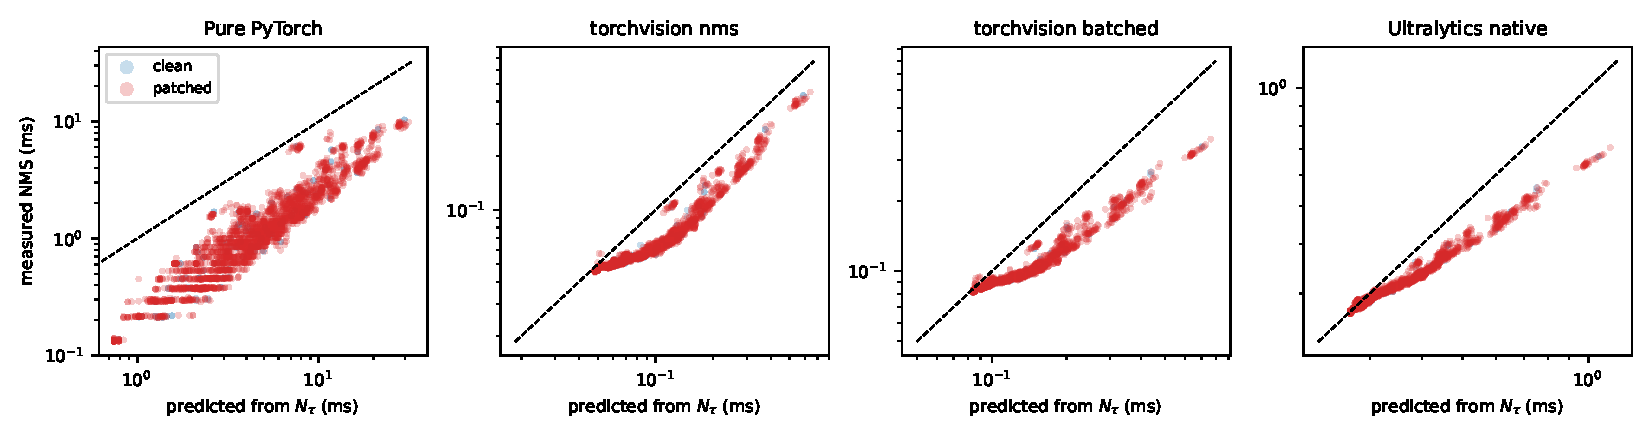
\includegraphics[width=\textwidth]{fig3_pred_vs_measured.pdf}
\caption{Độ trễ NMS đo được của các tập ứng viên thật ($\tau=0{,}01$, các điều kiện 320 px) so với dự đoán chỉ dựa trên $\Ntau$ từ đường cong đáp ứng liều hình học hỗn hợp, theo từng cách cài đặt. Đường nét đứt là đường bằng nhau. Điểm xanh là ảnh sạch, điểm đỏ là ảnh có patch (các điểm sạch ít và phần lớn bị che vì mỗi ảnh sạch chỉ là một điểm).}
\label{fig:pred}
\end{figure*}

\subsection{Kết quả trên điện thoại}
\label{sec:phone}
Chúng tôi dự định lặp lại hiệu chuẩn A/A và đối chứng dương trên điện thoại. Việc ghim lõi trên thiết bị được kiểm chứng dưới tải trên cụm lõi nhanh và cụm lõi chậm (các profile được định nghĩa trước khi chạy), và không profile nào qua kiểm chứng, nên không có phép đo thời gian nào được thực hiện và không có số liệu đáp ứng liều hay A/A nào được báo cáo cho điện thoại. Đây là một kết quả âm của giao thức ghim lõi trên thiết bị này chứ không phải một phát biểu về độ trễ của nó. Hệ quả là nhánh điện thoại của câu hỏi nghiên cứu không được trả lời ở đây; Mục~\ref{sec:threats} nêu đó là một hạn chế.

\section{Thảo luận}
\paragraph{Đối chứng dương xác lập điều gì.}
Giữa $10^2$ và $10^4$ ứng viên được tiêm, độ trễ NMS tăng từ 4 đến 1360 lần tùy cách cài đặt và hình học, và mức tăng được phát hiện ở MDE dưới 1,1\%. Vậy số ứng viên có ảnh hưởng đến thời gian NMS, nhưng mức ảnh hưởng phụ thuộc vào cách cài đặt NMS và vào cách các hộp chồng lấn; riêng $\Ntau$ không ấn định độ trễ. Kết quả vượt mốc (mọi lần lặp của pipeline PyTorch thuần với 2100 ứng viên đều vượt 100~ms) chỉ cho thấy bệ thử nghiệm có thể tạo ra một lần vượt mốc như vậy với cách cài đặt đó, không cho thấy một bộ phát hiện triển khai sẽ bị vượt mốc.

\paragraph{Nghiên cứu tình huống bổ sung điều gì.}
Hàm fitness của nghiên cứu tình huống không chứa thành phần độ trễ, nên mối liên hệ duy nhất của nó với độ trễ là giả định rằng $\Ntau$ theo sát độ trễ. Trong các phép đo của chúng tôi, câu trả lời là hỗn hợp. Giữa các ảnh, $\Ntau$ xếp hạng thời gian NMS tốt (tương quan hạng trên 0,84), và với baseline gradient thì thời gian NMS PyTorch thuần tăng 2,3 lần cùng với $\Ntau$. Tuy nhiên ở mức toàn bộ pipeline, cùng mức tăng 2,3 lần của $\Ntau$ làm thời gian toàn trình thay đổi ít hơn bề rộng khoảng tin cậy (1,006; khoảng 0,997 đến 1,015), vì bước lan truyền thuận chiếm phần lớn thời gian ở 320 px. Các patch của thuật toán di truyền không làm tăng $\Ntau$ đo được, và mức tăng thời gian 1 đến 1,5\% của chúng cũng có ở tìm kiếm ngẫu nhiên và ở các baseline. Do đó chúng tôi không thấy bằng chứng nào ở đây cho thấy việc cực đại hóa $\Ntau$ bằng bộ tối ưu này tạo ra tác động độ trễ, và kết quả ở 640 px vẫn còn bỏ ngỏ vì thiếu đường cơ sở sạch.

\paragraph{Hàm ý cho thực hành đánh giá.}
Báo cáo riêng $\Ntau$ không mô tả một tác động độ trễ. Một khẳng định về độ trễ cần đo thời gian theo công đoạn trên một profile đã ghim lõi và được kiểm chứng, một ước lượng A/A của sàn nhiễu, và cách cài đặt NMS cùng giới hạn mà pipeline triển khai dùng. Vì chi phí NMS phụ thuộc vào số hộp còn sống sót, các tấn công và phòng thủ nên được so sánh ở cùng hình học cũng như cùng $\Ntau$.

\paragraph{Cơ chế.}
Các phép đo phù hợp với mô hình chi phí ở Mục~\ref{sec:results} ở bốn khía cạnh. Thứ nhất, độ trễ NMS có tăng theo $\Ntau$ (H1), với hệ số phụ thuộc cách cài đặt. Thứ hai, hình học quyết định mức tăng bao nhiêu (H2): cài đặt dùng vòng lặp dành gần như toàn bộ thời gian cho các hộp được giữ lại, nên các hộp rời nhau tốn hơn hai bậc độ lớn so với một cụm dày đặc cùng kích thước. Thứ ba, giới hạn chặn chi phí (H3): tại $\Ntau=10^4$, giới hạn 300 làm giảm thời gian PyTorch thuần trên hộp rời nhau 72 lần và thời gian torchvision 650 lần. Thứ tư, phần chiếm của NMS trong pipeline quyết định việc thay đổi ở công đoạn NMS có nhìn thấy ở mức toàn trình hay không (H4). Điều mà mô hình chi phí không cung cấp là cách đổi $\Ntau$ thành mili giây: dự đoán chỉ dựa trên $\Ntau$ sai gấp bốn lần với cài đặt dùng vòng lặp, dù chỉ sai khoảng 5\% với cài đặt Ultralytics.

\paragraph{Vì sao bộ tối ưu của nghiên cứu tình huống không làm tăng $\Ntau$.}
Fitness huấn luyện cho thấy thuật toán di truyền gần như không cải thiện so với tìm kiếm ngẫu nhiên (Bảng~\ref{tab:train}), và fitness của nó bị chi phối bởi vị trí đặt patch hơn là cách chọn các pixel. Một patch 64 px phủ 4\% diện tích ảnh 320 px, và ngưỡng điểm 0,01 chấp nhận mọi anchor có chút bằng chứng về một đối tượng, nên số ứng viên chủ yếu do nội dung ảnh bên ngoài patch quyết định. Một phương pháp gradient bám theo gradient điểm số có thể nâng điểm của nhiều anchor cùng lúc và đạt số ứng viên gấp 2,3 lần; một tìm kiếm không dùng gradient với 625 lần đánh giá ứng viên không thể khám phá không gian đủ tốt. Đây là một quan sát về bộ tối ưu này và ngân sách này, không phải một phát biểu về tìm kiếm không gradient nói chung.

\paragraph{Quan hệ với các khẳng định trong tài liệu.}
Các mức tăng độ trễ được báo cáo của các tấn công NMS thường thu được với số lượng hộp lớn trên một nhân NMS dùng vòng lặp hoặc chạy trên GPU, trên một thiết bị biên cụ thể. Đối chứng dương của chúng tôi tái hiện khẳng định định tính trong một bối cảnh hẹp: với NMS dùng vòng lặp và hàng nghìn hộp rời nhau, độ trễ NMS tăng hai bậc độ lớn và thời gian toàn trình vượt mốc tham chiếu 100~ms. Cùng đối chứng đó cũng cho thấy bối cảnh này xa thực hành triển khai đến mức nào: với giới hạn 300 ứng viên, hiệu ứng giảm từ một đến ba bậc độ lớn, với một nhân thư viện phân biệt lớp thì giảm thêm, và với nội dung ảnh thực số ứng viên mà bộ tối ưu đạt được trên bộ phát hiện này thấp hơn số ứng viên được tiêm một đến hai bậc độ lớn (khoảng 90 so với $10^3$ đến $10^4$). Chúng tôi không đưa ra khẳng định nào về các bộ phát hiện hay thiết bị khác, và chúng tôi không kiểm tra các tấn công do các công trình được trích dẫn đề xuất. Kết quả của chúng tôi phù hợp với quan điểm rằng các tấn công độ trễ NMS cần một tổ hợp thuận lợi của cách cài đặt, giới hạn và hình học mới có ý nghĩa, một quan điểm mà EVADE lập luận từ một góc nhìn khác \cite{evade2025}.

\paragraph{Hướng dẫn cho đánh giá và phòng thủ.}
Với người đánh giá: báo cáo $\Ntau$ cùng cách cài đặt và giới hạn, đo từng công đoạn riêng, báo cáo sàn nhiễu A/A, và nêu mốc thời hạn nào đang được kiểm tra và vì sao. Với người phòng thủ: giới hạn số ứng viên trước NMS và một nhân thư viện có phân lô theo lớp là các thiết lập làm công đoạn NMS không nhạy với $\Ntau$ trong các phép đo của chúng tôi, và rẻ để áp dụng; bản thân việc chọn top-$k$ chỉ tốn một phần nhỏ của một mili giây. Với nhà nghiên cứu đề xuất một tấn công độ trễ: tối ưu độ trễ, hoặc một đại lượng thay thế mà quan hệ với độ trễ đã được kiểm chứng trên pipeline mục tiêu, và báo cáo hiệu ứng so với sàn nhiễu.

\paragraph{Điều gì có thể làm đổi kết luận của chúng tôi.}
Một bộ phát hiện lớn hơn trong đó NMS chiếm phần lớn hơn của pipeline, một độ phân giải khác (head thật ở 640 px có số anchor gấp bốn lần), một cách cài đặt có hằng số khác, hoặc một patch được tối ưu với thành phần độ trễ thay vì $\Ntau$ có thể tạo ra một tác động toàn trình mà nghiên cứu này không phát hiện được. Tác động của patch 640 px được để ngỏ cho đến khi đường cơ sở sạch 640 px được phân tích; khi được báo cáo, nó sẽ được báo cáo cùng sàn nhiễu riêng của nó (MDE toàn trình ở 640 px là 1,9\% với drift cao, Bảng~\ref{tab:aa}).

\section{Các mối đe dọa đối với tính hợp lệ}
\label{sec:threats}
Mục này tập hợp các hạn chế của nghiên cứu; các kết quả ở trên cần được đọc trong phạm vi các hạn chế này.

\paragraph{Tính hợp lệ nội tại.}
Mọi phép đo trên laptop đến từ một máy và một chế độ nguồn Windows; điện thoại duy nhất được chuẩn bị cho nghiên cứu không qua kiểm chứng ghim lõi. Nhiễu thời gian được định lượng bằng thiết kế A/A, nhưng phép đo tham chiếu bị lệch quá cờ 3\% ở 2/11 khối trong lần A/A 320 px (lớn nhất 26\%), 2/12 khối trong đối chứng dương (lớn nhất 5,6\%), 0/11 khối trong lần đo lại patch (lớn nhất 1,5\%), và 8/11 khối trong lần A/A 640 px (lớn nhất 18\%); các khối bị cờ được giữ trong phân tích chính và lần A/A có phân tích độ nhạy loại chúng. Điện thoại không ghim được, nên không có phép đo thời gian nào trên điện thoại. Các điều kiện patch ở 640 px chưa có nhánh sạch 640 px đã phân tích nên chưa đọc được như tác động độ trễ. Việc ghim lõi được kiểm chứng dưới tải, nhưng hệ điều hành vẫn có thể lập lịch công việc khác trên CPU đã ghim. Tập đo là 100 ảnh giữ ra ngoài, và tác động patch dùng năm trong mười seed tối ưu. Tập tối ưu và tập đo tách rời, và các patch được đóng băng bằng giá trị băm trước khi đo. Các phân tích định nghĩa sau khi xem dữ liệu được gắn nhãn post hoc.

\paragraph{Tính hợp lệ cấu trúc.}
$\Ntau$ là số anchor vượt ngưỡng trước NMS. Độ trễ được đo trên các tensor đã chuẩn bị trong bộ nhớ, nên không gồm giải mã ảnh, thu hình camera và truyền tải. Mốc tham chiếu 100~ms là giá trị do các tác giả chọn cho đối chứng dương, không phải yêu cầu của một ứng dụng. Các ứng viên tổng hợp có hình học và điểm số được kiểm soát mà các phát hiện thật có thể không có, và đó là lý do bộ dự đoán được kiểm tra trên các tập ứng viên thật. Vòng lặp NMS PyTorch thuần chậm hơn các nhân thư viện và khuếch đại sự phụ thuộc vào $\Ntau$; kết quả được báo cáo theo từng cách cài đặt chứ không gộp.

\paragraph{Tính hợp lệ bên ngoài.}
Nghiên cứu chỉ gồm một kiến trúc bộ phát hiện (YOLOv8n, float32) và một họ dữ liệu (COCO). Các bộ phát hiện hai giai đoạn, các bộ phát hiện không NMS như DETR \cite{carion2020detr}, các cỡ mô hình khác, mô hình lượng tử hóa và bộ tăng tốc không được bao phủ. Điện thoại là một SoC Arm chạy Ubuntu trong môi trường proot trên Android; nó không phải bo mạch nhúng, proot có thể thêm chi phí lời gọi hệ thống, và các bản dựng framework khác với laptop (PyTorch và Ultralytics mới hơn). Nếu thiết bị ghim được, chúng tôi sẽ so sánh tỷ số và hình dạng đường cong giữa các thiết bị và không bao giờ so độ trễ tuyệt đối. Các patch được chèn ở dạng số bằng các phép biến đổi phần mềm; không có đánh giá in-và-chụp hay qua camera nào được thực hiện.

\paragraph{Tính hợp lệ của kết luận.}
Các hiệu ứng được đọc so với MDE của A/A. Khoảng tin cậy chứa một, hoặc hiệu ứng dưới MDE, được báo cáo là không phát hiện ở độ nhạy đó và không được diễn giải là tương đương. Các phân tích patch có điều kiện trên các ảnh và seed đã lấy mẫu; bootstrap hai tầng tính đến cả hai nguồn biến thiên nhưng không tính đến các bộ phát hiện hay thiết bị khác. Các khoảng tin cậy không được hiệu chỉnh đa phép thử vì các phân tích là ước lượng chứ không phải một họ kiểm định.

\paragraph{Phạm vi của bộ tối ưu.}
Bộ tối ưu của nghiên cứu tình huống là hộp xám: nó đọc các điểm lớp trước NMS, thứ mà một dịch vụ triển khai thường không phơi bày, và nó không tối thiểu hóa độ trễ trực tiếp. Nghiên cứu không khẳng định một tấn công mạnh hơn các công trình trước, cũng không khẳng định một tấn công từ chối dịch vụ trên bất kỳ hệ thống triển khai nào.

\section{Kết luận}
Chúng tôi đã xem xét liệu số ứng viên trước NMS có dự đoán được độ trễ của bộ phát hiện không, bằng một giao thức kiểm chứng việc ghim lõi dưới tải và nêu hiệu ứng nhỏ nhất phát hiện được của mọi phép so sánh. Giữa $10^2$ và $10^4$ ứng viên được tiêm, độ trễ NMS tăng từ 4 đến 1360 lần tùy cách cài đặt và hình học, nên số ứng viên có ý nghĩa nhưng không quyết định độ trễ. Các patch của thuật toán di truyền được tối ưu trên 100 ảnh không làm tăng $\Ntau$ đo được ở 320 px và thêm 1 đến 1,5\% thời gian toàn trình, tương tự tìm kiếm ngẫu nhiên; một baseline gradient làm $\Ntau$ tăng 2,3 lần mà không có tác động toàn trình nhìn thấy được (khoảng 0,997 đến 1,015, MDE 0,55\%). Dự đoán chỉ dựa trên $\Ntau$ về thời gian NMS sai trong khoảng 5\% với NMS gốc Ultralytics nhưng sai gấp 4 lần với vòng lặp PyTorch thuần. Điện thoại không ghim được nên không có kết quả Arm, và tác động của patch 640 px đang chờ đường cơ sở sạch 640 px.

\section*{Phát hành có trách nhiệm}
Các sản phẩm được phát hành là bộ công cụ đo, các manifest, các fixture tiêm tổng hợp và các bản ghi thời gian thô. Các patch đã tối ưu không được đóng gói thành công cụ, và công việc giới hạn trong một bệ thử nghiệm cục bộ.

\section*{Sẵn có dữ liệu và mã}
Mã, các manifest kèm giá trị băm tệp và các bản ghi thời gian thô nằm trong kho mã của dự án \url{https://github.com/reikageisme/Sponge-patch-nms}. Kho chứa các tệp đăng ký trước cùng các tag quản lý phiên bản, bộ công cụ và các script phân tích, các manifest (ghi mã băm, phiên bản thư viện, cấu trúc CPU và chế độ nguồn), giá trị băm của mọi patch, các bản ghi thời gian thô của mọi lần chạy kể cả các lần bị loại, và các script sinh hình. Mọi con số trong các bảng truy được tới một selector trong tệp tóm tắt do một script trong kho tạo ra.

\section*{Tuyên bố sử dụng AI tạo sinh}
Một trợ lý lập trình AI (Claude Code) đã được dùng để giúp viết và kiểm thử bộ công cụ đo và để soạn thảo các phần của bản thảo. Các tác giả đặt giả thuyết và endpoint, chạy các phép đo, đối chiếu mọi con số được báo cáo với bản ghi thô, và chịu trách nhiệm về nội dung.

\section*{Tài trợ và xung đột lợi ích}
\paragraph{Tài trợ.} Nghiên cứu này không nhận tài trợ bên ngoài; đây là một dự án nghiên cứu độc lập của các tác giả.
\paragraph{Tuyên bố về xung đột lợi ích.} Các tác giả tuyên bố không có xung đột lợi ích.

\bibliographystyle{unsrtnat}
\bibliography{../paper_en/references}

\end{document}
